\documentclass{article}%
\usepackage{fancyhdr}
\usepackage[a4paper, top=2.5cm, bottom=2.5cm, left=2.2cm, right=2.2cm]%
{geometry}
\usepackage{amsmath}
\usepackage{changepage}
\usepackage{amssymb}
\usepackage{graphicx}%

\newenvironment{proof}[1][Proof]{\textbf{#1.} }{\ \rule{0.5em}{0.5em}}

\newcommand{\Q}{\mathbb{Q}}
\newcommand{\R}{\mathbb{R}}
\newcommand{\C}{\mathbb{C}}
\newcommand{\Z}{\mathbb{Z}}

\begin{document}

\title{Homework 3}
\author{Ted Xiao}
\date{\today}
\maketitle

\section{Basic Q-Learning Performance}
\begin{figure}[h]
    \center
		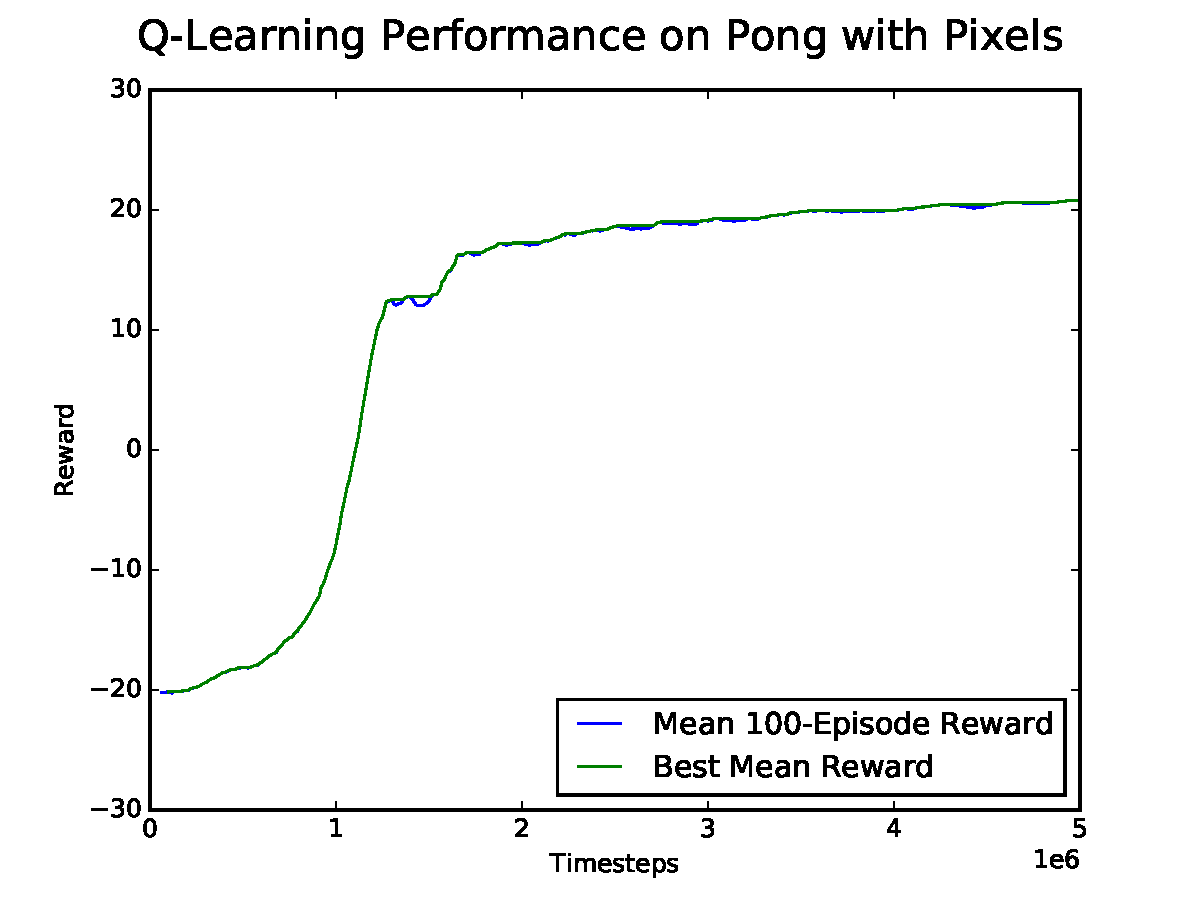
\includegraphics[width=0.6\textwidth]{lr1_images_plot.pdf}
    \caption{These results correspond to the default hyperparameters. It was run for 5 million timesteps on GPU.}
\end{figure}

\newpage
\section{Experimenting with Hyperparameters}

\begin{figure}[h]
  \centering
     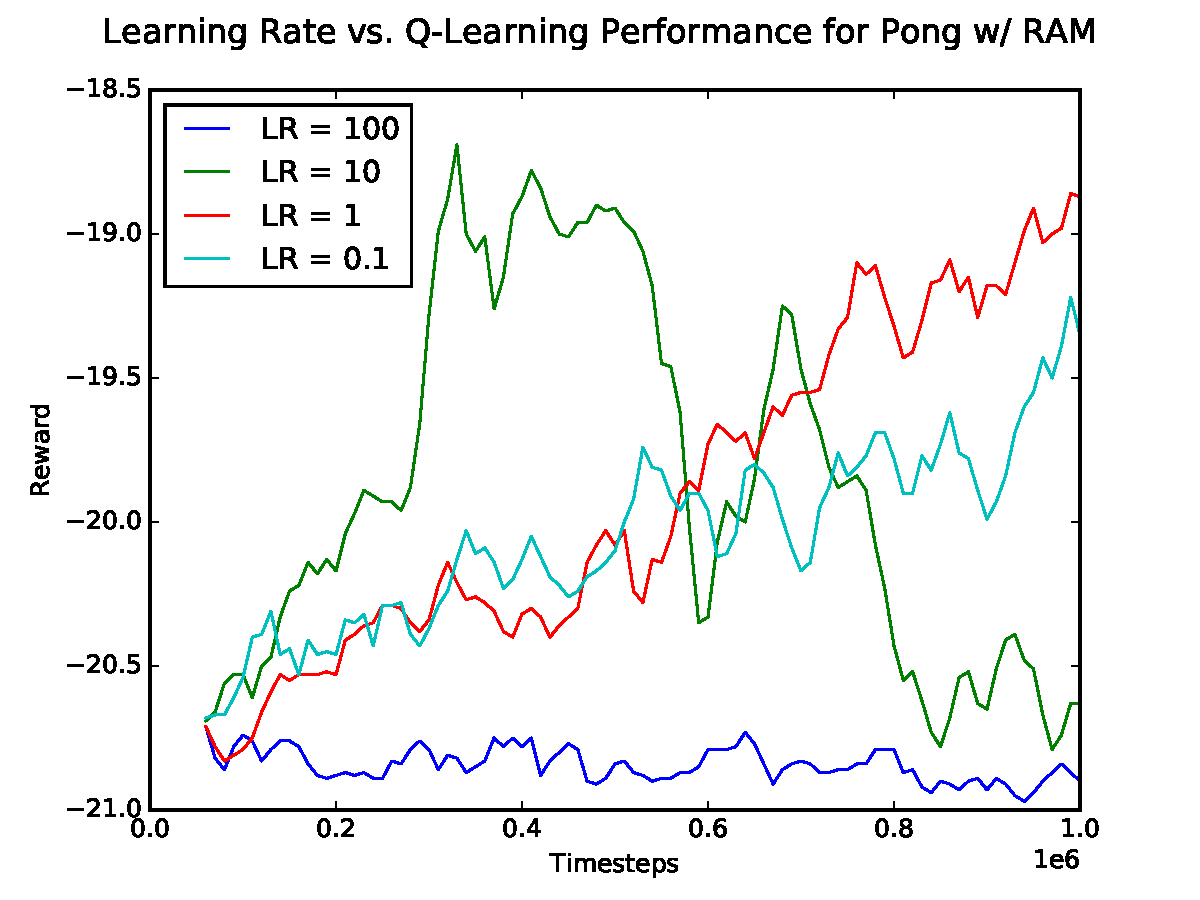
\includegraphics[width=0.9\textwidth]{lr_plot.pdf}
  \caption{The plot aboves shows the effect of learning rate on various trials of the Q-Learning model on Pong with RAM for 1 million steps. I chose to experiment with tuning learning rate (learning rate multiplier) because I was interested in comparing the sensitivity of exploration on Q-Learning with the sensitivity of learning rate on other tasks (Q-Value Iteration, Behavior Cloning). My intuition was that high learning rates would perform badly, and that seems to be the case. I was surprised that a LR of 10 was able to learn very quickly at first, which suggests that perhaps a scheduler that starts very high and decays fast might perform well.}
\end{figure}

\end{document}